% 
%% SOSP 2017 Template
%%
%% Uses sigplanconf from:
%% 
%%    http://www.sigplan.org/sites/default/files/sigplanconf.cls
%%
%% with 10pt and preprint options. 
%%
%% Replace 'XX' with your paper number (assigned when you register abstract)
%% Replace 'NN' with actual number of pages. 

\documentclass[10pt,preprint]{sigplanconf}
\usepackage{times}

\usepackage{datetime}
\usepackage{url}
\usepackage{hyperref}
\usepackage{graphicx}
\usepackage{xcolor}
\graphicspath{ {images/} }

\copyrightyear{2017} 


% These only appear when the 'preprint' option is specified.
% Enabling these will cause the first page of the document to fail the 
% format check on HotCRP :-(
%\titlebanner{Under submission to SOSP 2017 - do not cite or distribute}
%\preprintfooter{Draft of {\currenttime}, \today{}}

% No date in title area.
\date{}

% Paper number and no. of pages as author
\authorinfo{He Dai, Songhao Zhou}
		{Rice University}


% Actual document begins below.
\begin{document}

\title{Interesting Findings of Linux Message Queue/IPC} 
\maketitle

\begin{abstract}

We found four interesting topics when we prepared for the presentation and project of Linux Message Queue.

\end{abstract}

\section{Harsh Comments in Linux Source Code}

The comments in linux/ipc/syscall.c under ipc involves harsh words such as “horrible, ugly”.

System call is the services provided by Linux kernel. In C programming, it often uses functions defined in libc which provides a wrapper for many system calls. Internally, system call is invoked by software interrupt 0x80 to transfer control to the kernel. 

In linux/ipc/syscall.c, there’s a comments says “This is really horrible ugly, and new architectures should just wire up the individual syscalls instead”.

I’ve looked up the git commit history of this file in order to find out who wrote that comments. It turns out that although Christoph Hellwig was the one who committed the file back in 2010, he is not the one who wrote the comments. However, interesting point is the outcome of this comment.

Actually, I believe the syscall.c file is created because of the harsh comment since the functionality of syscall.c was scattered across a lot other kernel files (sys\_arm.c, sys\_cris.c,  sys\_frv.c, sys\_h8300.c, sys\_m32r.c, sys\_m68k.c, sys\_m68k.c, syscall.c, sys\_mn10300.c, syscalls.c, sys\_sh.c, sys\_sparc\_32.c). Because the nature of copy and paste on the same function across different files in the kernel makes it messy for other people to maintain the code which need to be updated multiple times whenever the function itself gets changed. Eventually, someone left that comment above all the old sys\_ipc() function to get other people’s attention and Christoph Hellwig took the action committed syscall.c to replace those redundant functions that spread across the kernel files.

Interesting enough, somehow Christoph Hellwig decided to keep the harsh comments when he created the syscall.c file in order to wire up the individual syscalls as the comments suggested. \\\\

\section{FIFO Implementation}

FIFO(also called named pipe) are commonly used for interprocess communication. \\
The main features of FIFO are:\\
1. It implements FIFO feature of the pipes\\
2. They can be opened just like normal files using their names\\
3. Data can be read from or written to the fifo\\
I tried to create a FIFO by Cygwin64 in Windows 10.\\
\subsection{Working with FIFO in a Shell}
Creating a FIFO\\
\colorbox{lightgray}{\begin{minipage}{8cm}
mkfifo
\end{minipage}}\\
Syntax\\
\colorbox{lightgray}{\begin{minipage}{8cm}
mkfifo [options] fifo\_name
\end{minipage}}\\
Example\\
\colorbox{lightgray}{\begin{minipage}{8cm}
\$ mkfifo fifo
\end{minipage}}\\
There is one more way by which we can FIFO using mknod. mknod is used to create block or character special files.\\
\colorbox{lightgray}{\begin{minipage}{8cm}
\$ mknod [OPTION]... NAME TYPE
\end{minipage}}\\
To create a FIFO fifo1\\
\colorbox{lightgray}{\begin{minipage}{8cm}
\$ mknod fifo1 p
\end{minipage}}\\
where p corresponds to file type : pipe (remember FIFO is a named pipe).\\

\subsection{Reading/ Writing data from/to a FIFO}
Let’s open two terminals.\\
In the first terminal:\\
\colorbox{lightgray}{\begin{minipage}{8cm}
\$ cat $>$ fifo
\end{minipage}}\\
we are experimenting with the FIFO. This is second line. After opening the fifo in the second terminal for readingusing cat, you will notice the above two lines displayed there.
Now open the second terminal and go to the directory containing the FIFO ‘fifo’\\
\colorbox{lightgray}{\begin{minipage}{8cm}
\$ cat $<$ fifo
\end{minipage}}\\
we are experimenting with the FIFO. This is second line. After opening the fifo in the second terminal for reading
Now keep on writing to the first terminal. You will notice that every time you press enter, the corresponding line appears in the second terminal.\\
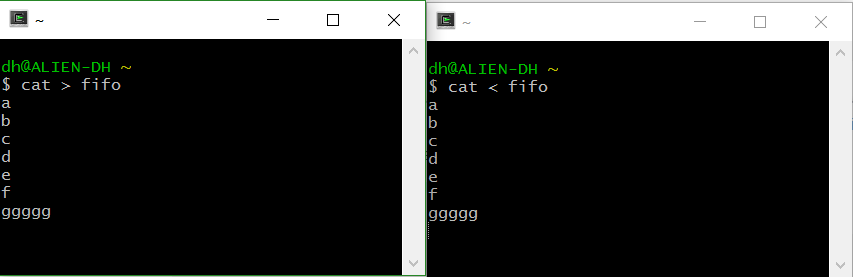
\includegraphics[totalheight=27mm]{fig1.png}
Pressing CTRL+D in the first terminal terminates writing to the fifo. This also terminates the second process because reading from the fifo now generates a “BROKEN PIPE” signal. The default action for this is to terminate the process.\\
Let us now see the details of the file ‘fifo’:\\

\includegraphics[totalheight=7mm]{fig2.png}\\
The p in the beginning denotes that it is a pipe.\\
Let’s see more details about the pipe using stat:\\
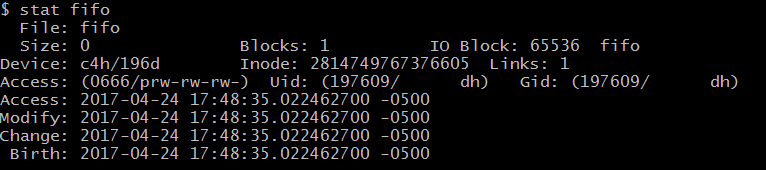
\includegraphics[totalheight=18mm]{fig3.png}\\
If you notice carefully, FIFOs just like a normal file possess all the details like inode number, the number of links to it, the access, modification times, size and the access permissions.\\
As in the case of pipes, there alos can be multiple readers and writers to a pipe. Just try open multiple terminals to read from and write to a pipe.\\\\

\section{IPC spin locks in multicore system}

IPC was using semaphore to manage accessing the shared memory instead of using spin  
Locks in System V IPC. But later on IPC introduces the option using spin locks.

The main reason is that back in the days when System V IPC was introduced there were not many multicore systems. 

Because of the nature of spin locks, when a thread tries to lock a spinlock and it does not succeed, it will continuously re-try locking it, until it finally succeeds. It will not allow another thread to take its place.

Thus, using spinlocks on a single-core/single-CPU system usually makes no sense because as long as the spinlock polling is blocking the only available CPU core, no other thread can run and since no other thread can run, the lock won't be unlocked either. 

Instead, If the thread was put to sleep instead, another thread could have ran at once, possibly unlocking the lock and then allowing the first thread to continue processing, once it woke up again. This is exactly the case when a thread tries to lock a semaphore and it does not succeed, because the semaphore is already locked, it will go to sleep, immediately allowing another thread to run. It will continue to sleep until being woken up. And i believe this led System V IPC ended up with implementing using semaphore as in linux/ipc/sem.c file. 

However, things changed as multicore system gradually becomes a standard. IPC gives programmers the option to use spin\_lock\_irq in linux/ipc/shm.c file.\\\\

\section{Message Queue from System V to POSIX}

System V is used from Old version of Unix system operating system API. POSIX (Portable Operating System Interface Unix) is meant to be new portable implementation of API created after during Unix War. POSIX is supposed to be thread safe and is relatively advanced but still System V is used widely.\\
Both System V IPC (XSI IPC) and POSIX IPC including three different mechanisms for inter-processes communication:
\begin{itemize}
	\item Message queues: pass messages between processes
	\item Semaphores: synchronize for multiple processes by kernel
	\item Shared memory: share region of memory
\end{itemize}
Message queues were added by the POSIX realtime standard 1003.1b-1993. The interface for POSIX message queues is different from System V message queues, and should not be confused. POSIX message queue interface commands begin with the prefix "mq\_" (i.e. mq\_open(), etc), and the interface can be found in $<$mqueue.h$>$. And System V message queue is uniquely identified by a positive integer (its msqid) and has an associated data structure of type struct msqid\_ds, defined in $<$sys/msg.h$>$

I would think that the older API (System V) would have had more time to be performance tuned, but that's just speculation which is of course no substitute for real-world testing.

As to why there are two standards -- POSIX created their standard because they thought it was an improvement on the System V standard. But if everyone agreed that POSIX IPC is better, many many many programs still use System V IPC(Like Versions of Cygwin prior to 1.7 didn't even support POSIX IPC until 2009, right now is still optional library) and it would take years to port them all to POSIX IPC. In practice, it would not be worth the effort so even if all new code used POSIX IPC as of tomorrow, System V IPC would stick around for many years.

\bibliographystyle{acm}
% \bibliography{xxx}

\end{document}
